
\chapter{Agricultural Robot System}

This chapter describes the design and functioning of an agricultural robot that autonomously navigates, detects diseases and pests, and sprays chemicals using advanced technologies such as Gaussian splatting and convolutional neural networks (CNNs). The robot is constructed with aluminum extrusion as its frame, motors for movement and arm control, and various sensors and components for navigation and operation. An Android application is used to control both the Arduino Uno and the ESP32 microcontrollers for precise movement and spraying actions.

\section{System Overview}

The robot uses a mobile phone, specifically a Google Pixel, as its primary processing unit. \cite{müller2021openbotturningsmartphonesrobots} The phone's camera captures images to create a 3D Gaussian splat map for navigation, allowing the robot to identify its position in the field and locate target objects for spraying. Additionally, the robot is capable of identifying diseases and pests using a CNN-based model trained on agricultural datasets. The system operates as follows:

\begin{enumerate}
    \item The robot wakes up and captures an image using the phone's camera.
    \item The image is processed to create a 3D Gaussian splat for localization and mapping.\cite{chen2024splatnavsaferealtimerobot} \cite{bortolon20246dgs6dposeestimation}
    \item Simultaneously, the image is analyzed using a CNN-based model to detect diseases or pests on plants.\cite{10353343}
    \item Based on the identified location and any detected issues, the robot receives instructions to move to a specific point.\cite{DURAKLI2022101540}
    \item Using OpenVLA, the robot performs actions such as moving its arms and spraying chemicals on the target objects. \cite{kim2024openvlaopensourcevisionlanguageactionmodel}
\end{enumerate}

The system connects to the web server to send images, receive instructions for navigation, and apply actions based on disease and pest identification. An Android application is also used to control the robot’s movement and spraying mechanism, providing a user-friendly interface for manual control when needed.

\section{Communication and Control}
The Android phone uses USB-C to serial adapter to communicate with the Arduino Uno and ESP32 microcontrollers. The Arduino Uno controls the motors for arm movement and the hydraulic motor for spraying, while the ESP32 controls the base wheel motors for navigation. The phone captures images and sends them to the cloud server for processing, receiving navigation instructions and action tokens in return. The robot's operation is coordinated through a combination of image processing, navigation algorithms, and disease/pest detection logic.


\section{Gaussian Splatting for Navigation and Mapping}

Gaussian splatting offers an innovative approach to real-time navigation, mapping, and semantic understanding by transforming sparse 3D point clouds into continuous Gaussian distributions (splats). This technique provides an efficient representation of the environment, enabling the robot to perform real-time updates and optimizations for navigation tasks.

The key components of Gaussian splatting include:
\begin{itemize}
    \item \textbf{GSplat Reconstruction:} The robot converts images captured by the camera into 3D Gaussian splats, forming a geometric representation of the environment. This allows the robot to optimize navigation in real-time. \cite{chen2024splatnavsaferealtimerobot}
    \item \textbf{Pose Estimation:} Using the Gaussian splat map, the robot performs pose estimation to accurately determine its position in the field. \cite{bortolon20246dgs6dposeestimation}
    \item \textbf{Path Planning:} The robot plans its path by constructing polytopic safe corridors, ensuring collision-free navigation.\cite{DURAKLI2022101540}
    \item \textbf{Motion Control:} The planned trajectory is executed through smooth motion control, integrated with the Gaussian splat environment for dynamic adjustments during navigation.\cite{DURAKLI2022101540}
\end{itemize}

This approach enables the robot to navigate autonomously in complex agricultural environments, continuously refining its internal map as it moves through the field.


\section{Electronics and Control System}

The robot's electronics are controlled by an Arduino Uno, which drives the motors in the arms. The power system consists of an S4 9V battery, which is converted to 12V using a voltage converter. The motor control is achieved using TMC2208 drivers, providing smooth and precise control of the arm motors.

The base wheel motors are powered by a separate battery, identical to the one used for the arms. The ESP32 microcontroller, along with a relay, controls the motors and ensures proper movement of the robot. The hydraulic motor for the spraying mechanism is also controlled by the Arduino Uno.

\section{Hydraulic System}
The hydraulic system of the robot consists of a pump, a reservoir, and a spraying mechanism. The pump is powered by a separate power supply, providing the necessary pressure to drive the liquid spraying system. The reservoir holds the chemicals to be sprayed, which are released through the spraying mechanism when activated. The hydraulic system is controlled by the Arduino Uno, ensuring precise and efficient spraying of chemicals on target objects.

\cite{azghadi2024preciseroboticweedspotspraying}

\subsection{Power System}

The power system of the robot consists of:

\begin{itemize}
    \item An S4 9V battery for the arm motors and control system.
    \item A voltage converter to step up the voltage to 12V for motor operation.
    \item TMC2208 motor drivers to control the NEMA 17 motors.
    \item A separate S4 9V battery for the base wheel motors.
    \item Power supply for the hydraulic motor to drive the liquid spraying system.
    \item Hydraulic pump and reservoir for chemical spraying using a Relay.
\end{itemize}

\section{Software and Communication}

The robot's software is based on a combination of image processing, navigation algorithms, disease/pest detection, and motor control logic. The mobile phone serves as the main computational brain, performing the following tasks:

\begin{itemize}
    \item Capturing images for localization and disease/pest detection.
    \item Sending images to the cloud server to create a 3D Gaussian splat map.
    \item Analyzing images using the CNN model to detect diseases and pests.
    \item Receiving instructions from the server based on the identified location and detected issues.
    \item Using OpenVLA to generate action tokens for arm movement and spraying.
\end{itemize}

The ESP32 microcontroller is responsible for controlling the base motors, using feedback from an accelerometer to maintain stability and ensure accurate navigation. The Android application provides manual control over the robot, enabling the user to issue movement commands or activate the spraying mechanism when needed.

\section{Operation Workflow}

The robot operates autonomously in the field with the following workflow:

\begin{enumerate}
    \item The robot powers on and initializes all systems.
    \item The mobile phone captures an image of the surroundings.
    \item The image is sent to the cloud server for localization using Gaussian splatting.
    \item Simultaneously, the image is analyzed for disease and pest detection using a CNN model.
    \item The robot receives navigation instructions and moves to the specified location.
    \item The arms are positioned based on action tokens generated by OpenVLA.
    \item The spraying mechanism is activated using the hydraulic motor, and chemicals are applied to the target object if diseases or pests are detected.
    \item The user can also manually control the robot's movement and spraying mechanism using the Android app.
\end{enumerate}

\section{IK and FK for Arm Movement}

The robot's arm movement is controlled using Inverse Kinematics (IK) and Forward Kinematics (FK) algorithms. The IK algorithm calculates the joint angles required to position the end effector at a specific location, while the FK algorithm determines the end effector's position based on the joint angles. These algorithms enable precise and efficient control of the robot's arms, allowing it to perform complex tasks such as spraying chemicals on target objects.
Using a grid based system with the image segmentation, the robot can identify the location of the target object and calculate the IK and FK to move the arm to the desired position.


\section{Workflow Diagram}

\begin{figure}[h]
    \centering
    \begin{tikzpicture}[node distance=2cm]
        % Define block styles
        \tikzstyle{process} = [rectangle, rounded corners, minimum width=3cm, minimum height=1cm, text centered, draw=black, fill=orange!30]
        \tikzstyle{decision} = [diamond, minimum width=3cm, minimum height=1cm, text centered, draw=black, fill=green!30]
        \tikzstyle{io} = [trapezium, trapezium left angle=70, trapezium right angle=110, minimum width=3cm, minimum height=1cm, text centered, draw=black, fill=blue!30]
        \tikzstyle{arrow} = [thick,->,>=stealth]
        
        % Nodes
        \node (start) [process] {Robot Powers On};
        \node (image) [process, below of=start] {Capture Image};
        \node (cloud) [process, below of=image] {Send Image to Cloud for GSplat};
        \node (detection) [process, right of=cloud, xshift=5cm] {Disease/Pest Detection via CNN};
        \node (server) [process, below of=cloud] {Receive Navigation Instructions};
        \node (move) [process, below of=server] {Move to Location};
        \node (arms) [process, below of=move] {Move Arms Based on Tokens};
        \node (spray) [process, below of=arms] {Activate Spraying Mechanism};
        
        \node (manual) [decision, right of=move, xshift=4cm] {Manual Control?};
        \node (android) [io, below of=manual, xshift=4cm] {Android App Controls Movement and Spraying};
        
        % Arrows
        \draw [arrow] (start) -- (image);
        \draw [arrow] (image) -- (cloud);
        \draw [arrow] (cloud) -- (server);
        \draw [arrow] (server) -- (move);
        \draw [arrow] (move) -- (arms);
        \draw [arrow] (arms) -- (spray);
        
        \draw [arrow] (image.east) -- ++(3,0) |- (detection);
        \draw [arrow] (detection) -- (spray);
        
        \draw [arrow] (move.east) -- ++(1.5,0) |- (manual);
        \draw [arrow] (manual) -- (android);
        \draw [arrow] (android.west) -- ++(-2.5,0) |- (arms);
    \end{tikzpicture}
    \caption{Workflow of the Agricultural Robot System}
\end{figure}

\begin{figure}[h]
    \centering
    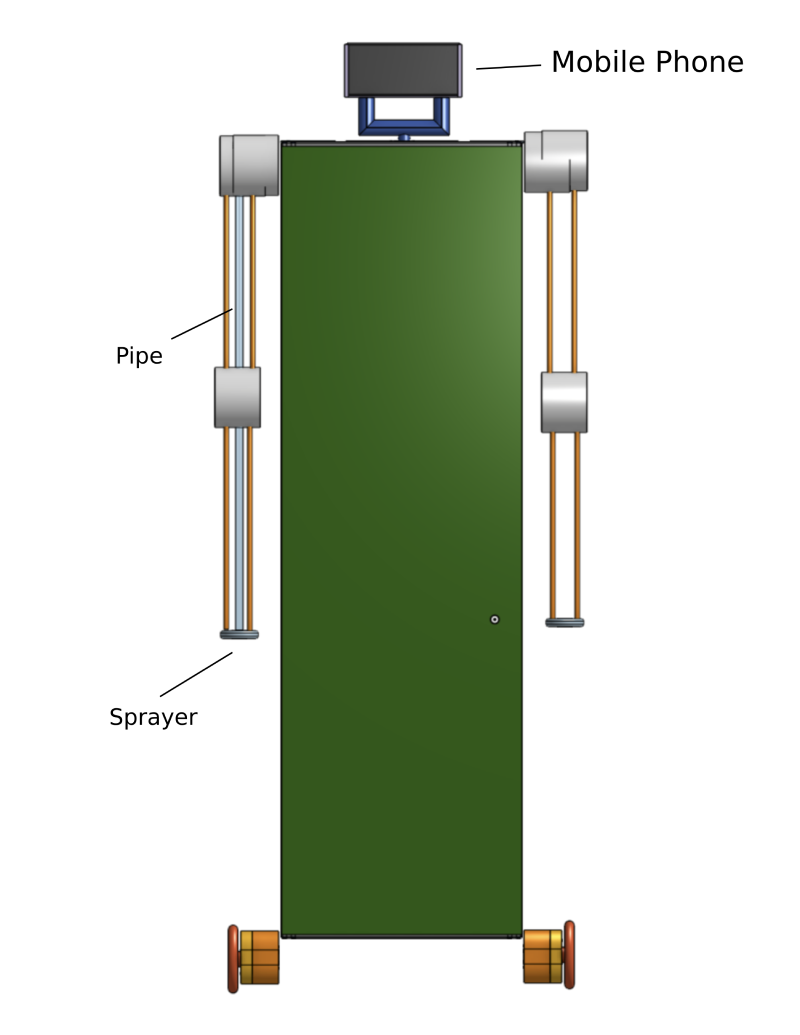
\includegraphics[width=0.8\textwidth]{robot.png}
    \caption{Diagram of the Agricultural Robot}
\end{figure}

\begin{figure}[h]
    \centering
    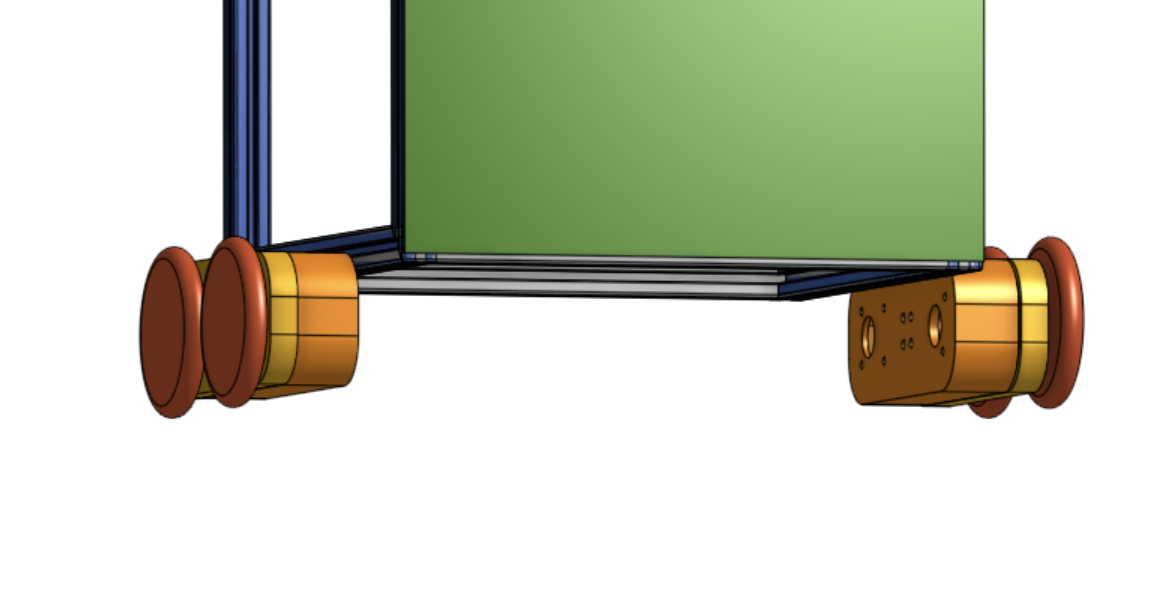
\includegraphics[width=0.8\textwidth]{legs.png}
    \caption{Wheels of the Agricultural Robot}
\end{figure}

\begin{figure}[h]
    \centering
    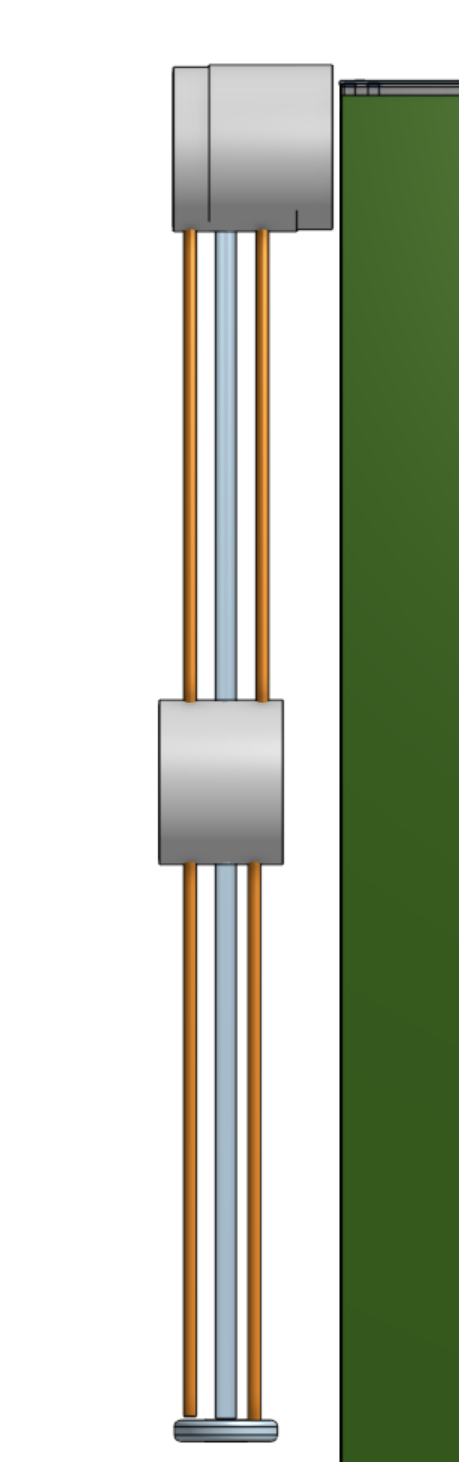
\includegraphics[height=0.3\textwidth]{arm.png}
    \caption{Arm of the Agricultural Robot}
\end{figure}

\section{Tools Used}

The following tools were used in the development of the agricultural robot system:

\begin{itemize}
    \item \textbf{Arduino Uno:} Controls the arm motors and hydraulic motor.
    \item \textbf{ESP32:} Controls the base wheel motors for navigation.
    \item \textbf{Google Pixel:} Acts as the main processing unit for image capture and analysis.
    \item \textbf{Android App:} Provides manual control over the robot's movement and spraying mechanism.
    \item \textbf{OpenVLA:} Generates action tokens for arm movement and spraying based on visual and language inputs.
    \item \textbf{Gaussian Splatting:} Creates a 3D Gaussian splat map for navigation and mapping.
    \item \textbf{CNN Model:} Detects diseases and pests in plants from captured images.
    \item \textbf{Hydraulic System:} Sprays chemicals on target objects based on detected issues.
    \item \textbf{IK and FK Algorithms:} Control the arm movement for precise positioning.
    \item \textbf{Grid Based System:} Identifies the location of target objects for arm movement.
    \item \textbf{Image Segmentation:} Analyzes images to detect diseases and pests in plants.
    \item \textbf{Web Server:} Communicates with the robot to provide navigation instructions and action tokens.
    \item \textbf{Voltage Converter:} Steps up the voltage to 12V for motor operation.
    \item \textbf{TMC2208 Motor Drivers:} Control the NEMA 17 motors for smooth and precise movement.
    \item \textbf{Relay:} Controls the hydraulic motor for spraying chemicals on target objects.
    \item \textbf{Accelerometer:} Provides feedback for maintaining stability during navigation.
    \item \textbf{CAD - Onshape} Used for designing the robot and its components.
    \item \textbf{Python:} Programming language used for developing the robot's software.
    \item \textbf{FastAPI:} Web framework used for creating the REST API for communication.
    \item \textbf{Orca Slicer:} Used for slicing the 3D models for printing.
    \item \textbf{Ender 3:} 3D printer used for printing the robot's components.
    \item \textbf{S4 9V Battery:} Power source for the arm motors and control system.

\end{itemize}
